\section{Control flow graph}
\tikzstyle{subtree} = [rectangle, draw, fill=gray!20, text width=4em, text badly centered, minimum height=3em]
\tikzstyle{node} = [draw, circle, minimum height=2em]
\tikzstyle{emptynode} = [draw, circle]
\tikzstyle{line} = [draw, -latex']
\tikzstyle{entry} = [draw=none,fill=none]
\tikzstyle{exit} = [draw=none,fill=none]
\tikzstyle{dots} = [draw=none,fill=none]
\newcommand{\subt}[1]{\llbracket #1\rrbracket}

Given a P0 program, $p : \syn{program}$, parsed to a abstract syntax tree, the control flow graph can be constructed recursively where every graph has an entry and an exit node. Most of the nodes takes arguments. Here $h$ denotes variables of type HeapTemps, $t$ variables of type Temps, and $c$ variables of either type. Subgraphs are denoted by a grey rectangles with letters $\subt{S}$, $\subt{E}(t)$, $\subt{R}(h)$, $\subt{V}(h)$, and $\subt{T}(c)$ which denotes subgraph of statement $S$, expression $E$ with the resulting value stored in variable $t$, reference expression $R$ with resulting heap-location-set stored in $h$, variable expression $V$ with resulting heap-location-set stored in $h$, or either expression with the result stored in $c$ respectively. For a given argument, $c$, to the subgraph, the variable corresponds to the target variable, $c_{tar}$, in the subgraph. E.g. the expression \texttt{1+(2+3)} becomes graph \ref{graph:exexpr}.
\begin{graph}
\centering
\begin{adjustbox}{max size={.25\textwidth}{.25\textheight}}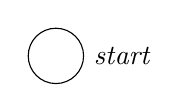
\begin{tikzpicture}[node distance = 2cm, auto]
    % Place nodes
    \node [node, label={0:$\mathit{start}$}] (if) {};
 
    % Draw edges
%    \path[line] (en) -> (e1);
 
\end{tikzpicture}\end{adjustbox}
\caption{Example graph of expression \texttt{1+(2+3)}}
\label{graph:exexpr}
\end{graph}
The control-flow graph created from $p$ starts with a $\mathit{start}$ node followed by the control-flow graphs for each statement in $p$, connected edges from exit to entry nodes, in the order of appearance. 

For each function definition encountered a separate graph is created, which may later be referenced. This graph starts with a $\mathit{start}$ node and ends with an $\mathit{exit}$ node, between these are the graph corresponding to the function body. The arguments of the exit node are the temporary variables created by the return statements. 

\subsection{Statements}
Let $s : \syn{statement}$ be a statement, then there are nine different graphs, one for each case in the grammar \ref{gramm:p0}. The first four, for $s = $ \texttt{while($E$) $S$}, $s = $ \texttt{for($E_1$;$ E_2$;$E_3$) $S$}, $s = $ \texttt{if($E$) $S$}, and $s = $ \texttt{if($E$) $S_1$ else $S_2$} statements, are depicted as graph \ref{graph:flowwhile}, \ref{graph:flowfor}, \ref{graph:flowif}, and \ref{graph:flowifelse} respectively.


\begin{graph}
\hspace*{\fill}
\subcaptionbox{\label{graph:flowwhile}}{\begin{adjustbox}{max size={.25\textwidth}{.25\textheight}}\begin{tikzpicture}[node distance = 2cm, auto]
    % Place nodes
    \node [entry] (en) {};
    \node [subtree, below of=en] (e1) {$\subt{E}(t)$};
    \node [node, below of=e1, label={0:$\mathit{if}(t)$}] (if) {};
    \node [subtree, below of=if ] (s1) {$\subt{S}$};
    \node [emptynode, below of=s1 ] (end) {};
    \node [exit, below of=end] (ex) {};

    % Draw edges
    \path[line] (en) -> (e1);
    \path [line] (e1) -> (if);
    \path [line] (if) -> (s1);
    \path [line] (if) -- (-2, -4) |- (end); 
    \path [line] (s1) -- (2, -6) |- (e1); 
    \path [line] (end) -> (ex);
\end{tikzpicture}\end{adjustbox}}\hfill%
\subcaptionbox{\label{graph:flowfor}}{\begin{adjustbox}{max size={.25\textwidth}{.25\textheight}}\begin{tikzpicture}[node distance = 2cm, auto]
    % Place nodes
    
    \node [entry] (en) {};
    \node [subtree, below of=en] (e1) {$\subt{E_1}(\_)$};
    \node [subtree, below of=e1] (e2) {$\subt{E_2}(t)$};
    \node [node, below of=e2, label={135:$\mathit{if}(t)$}] (if) {};
    \node [subtree, below left of=if] (s) {$\subt{S}$};
    \node [subtree, below right of=if] (e3) {$\subt{E_3}(\_)$};
    \node [emptynode, below right of=s] (end) {};
    \node [exit, below of=end] (ex) {};
    
    % Draw edges
    \path [line] (en) -> (e1);
    \path [line] (e1) -> (e2);
    \path [line] (e2) -> (if);
    \path [line] (if) -> (s);
    \path [line] (s) -> (e3);
%    \path [line] (e3) -> (end);
    \path [line] (end) -> (ex);
    \path [line] (e3) |- (e2);
    \path [line] (if) -- (-3, -6) |- (end);
\end{tikzpicture}\end{adjustbox}}\hfill%
\subcaptionbox{\label{graph:flowif}}{\begin{adjustbox}{max size={.25\textwidth}{.25\textheight}}\begin{tikzpicture}[node distance = 2cm, auto]
    % Place nodes
    
    \node [entry] (en) {};
    \node [subtree, below of=en] (e1) {$\subt{E}(t)$};
    \node [node, below of=e1, label={45:$\mathit{if}(t)$}] (if) {};
    \node [subtree, below of=if] (s1) {$\subt{S}$};
    \node [emptynode, below of=s1](end) {};
    \node [exit, below of=end] (ex) {};
    
    % Draw edges
    \path [line] (en) -> (e1);
    \path [line] (e1) -> (if);
    \path [line] (if) -> (s1);
    \path [line] (s1) -> (end);
    \path [line] (if) -- (2,-4) |-  (end);
    \path [line] (end) -> (ex);
\end{tikzpicture}\end{adjustbox}}\hfill%
\subcaptionbox{\label{graph:flowifelse}}{\begin{adjustbox}{max size={.25\textwidth}{.25\textheight}}\begin{tikzpicture}[node distance = 2cm, auto]
    % Place nodes
    \node [entry] (en) {};
    \node [subtree,below of=en] (e1) {$\subt{E}(t)$};
    \node [node, below of=e1, label={35:$\mathit{if}(t)$}] (if) {};
    \node [subtree, below left of=if] (s1) {$\subt{S_1}$};
    \node [subtree, below right of=if] (s2) {$\subt{S_2}$};
    \node [emptynode, below right of=s1](end) {};
    \node [exit, below of=end] (ex) {};
    % Draw edges
    \path[line] (en) -> (e1);
    \path [line] (e1) -> (if);
    \path [line] (if) -> (s1);
    \path [line] (if) -> (s2);
    \path [line] (s1) -> (end);
    \path [line] (s2) -> (end);
    \path [line] (end) -> (ex);
\end{tikzpicture}\end{adjustbox}}
\hspace*{\fill}
\end{graph}

%For $s =$ \texttt{global $v_1,\cdots, v_n$} the graph is containing a single, $global$, node which takes the variable names $v_1,\cdots v_n$ as argument. 
Return-statements, $s =$ \texttt{return $T$} have three different graphs. If the return statement is empty, i.e. does not contain an expression, then this is equivalent of returning \texttt{null}, this case yields the graph in \ref{graph:floweret}. If $T : \syn{rexpr}$ and the function is a reference function, i.e. the function signature has an ampersand before the function name, then the references is returned (graph \ref{graph:flowret} where $c : \text{HeapTemps}$). If this is not the case, assuming the program is a valid P0 program, then it is fair to assume that $T$ can be parsed as an expression, since it cannot be an array-append operation. If it was an array append operation, then the program wouldn't be a valid PHP program and thus not a valid P0 program (see section \ref{sec:langsubset}). Assuming that the $T : \syn{expr}$ the graphs for a return statement should evaluate $T$ and return the result, this is the case in graph \ref{graph:flowret} with $c : \text{Temps}$.  For all graphs, the exit-node is the unique exit-node of the function.

\begin{program}
 \begin{subfigure}[b]{.45\linewidth}
	\begin{lstlisting} 
	\end{lstlisting}
    \caption{Normal return-statement}
  \end{subfigure}\hfill%
 \begin{subfigure}[b]{.45\linewidth}
	\begin{lstlisting} 
	\end{lstlisting}
    \caption{Reference return-statement}
  \end{subfigure}

\caption{Return-statement examples}
\label{lst:return-statements}
\end{program}

\begin{graph}

\hspace*{\fill}
\subcaptionbox{\label{graph:floweret}}{\begin{adjustbox}{max size={.3\textwidth}{.25\textheight}}\begin{tikzpicture}[node distance = 2cm, auto]
    % Place nodes
    \node [entry] (en) {};
    \node [node, below of=en, label={45:$\mathit{const}_r(\texttt{null}, t_{tar})$}] (const) {};
    \node [node, below of=const, label={45:$\mathit{exit}(\cdots, t_{tar}, \cdots)$}] (exitn) {};
    \node [emptynode, below of=exitn ] (end) {};
    \node [exit, below of=end] (ex) {};
      % Draw edges
    \path[line] (en) -> (const);
    \path[line] (const) -> (exitn);
    \path[line] (end) -> (ex);
    
\end{tikzpicture}\end{adjustbox}}\hfill%
\subcaptionbox{\label{graph:flowret}}{\begin{adjustbox}{max size={.3\textwidth}{.25\textheight}}\begin{tikzpicture}[node distance = 2cm, auto]
    % Place nodes
    \node [entry] (en) {};
    \node [subtree, below of=en] (exp) {$\subt{T}(c)$};
    \node [node, below of=exp, label={45:$\mathit{exit}(\cdots, c, \cdots)$}] (exitn) {};
    \node [emptynode, below of=exitn ] (end) {};
    \node [exit, below of=end] (ex) {};
    % Draw edges
    \path[line] (en) -> (exp);
    \path[line] (exp) -> (exitn);
    \path[line] (end) -> (ex);
    
\end{tikzpicture}\end{adjustbox}}
\hspace*{\fill}
\end{graph}

The remaining four graphs are the empty graph, the graph of the expression statement, the graph of \texttt{global} statement, and the graph of the block statement which are all straight-foward.


\subsection{Expressions}

Let $e : \syn{expr}$ then, by ignoring the trivial parenthesized expression case, viewing the four increment/decrement operations as one, and the two array-initialization operations as one, the expression can be on nine different forms. For $e = E_l \oplus E_r$ the graph depends on the operation. If the operation is a short-circuit operation, logical \texttt{\&\&} or \texttt{||}, then the graph is as \ref{graph:flowsop} because only one branch may be required to be evaluated. If the operation is not a short-circuit operation then the graph becomes as \ref{graph:flowbop}, because both expressions must be evaluated. In both cases the operations are performed on, and saved in, the temporary storage. The unary operation, $e = \circ E$ is similar to the previous case with a graph as \ref{graph:flowuop}. A separate graph for unary post/pre increment/decrement operations are necessary because of the performed update on the heap location. This is the reason for the operations not being performed on the temporary storage, but instead on heap-locations directly. The result of the operation is stored in the temporary storage. Figure \ref{graph:flowinc} illustrates the corresponding flow graph.
\begin{graph}
\hspace*{\fill}
\subcaptionbox{\label{graph:flowsop}}{\begin{adjustbox}{max size={.24\textwidth}{.25\textheight}}\begin{tikzpicture}[node distance = 2cm, auto]
    % Place nodes
    \node [entry] (en) {};
    \node [subtree, below of=en] (e1) {$\subt{E_l}(t_l)$};
    \node [node, below of=e1, label={0:$\mathit{if}(t_l)$}] (if) {};
    \node [subtree, below of=if] (e2) {$\subt{E_r}(t_r)$};
    \node [node, below of=e2, label={0:$\mathit{sop}_\oplus(t_l,t_r,t_{tar})$}] (sop) {};
    \node [exit, below of=sop] (ex) {};

    % Draw edges
    \path [line] (en) -> (e1);
    \path [line] (e1) -> (if);
    \path [line] (if) -> (e2);
    \path [line] (e2) -> (sop);
    \path [line] (if) -- (-2, -4) |- (sop);
    \path [line] (sop) -> (ex);
\end{tikzpicture}\end{adjustbox}}\hfill%
\subcaptionbox{\label{graph:flowbop}}{\begin{adjustbox}{max size={.24\textwidth}{.25\textheight}}\begin{tikzpicture}[node distance = 2cm, auto]
    % Place nodes
    \node [entry] (en) {};
    \node [subtree, below of=en] (e1) {$\subt{E_l}(t_l)$};
    \node [subtree, below of=e1] (e2) {$\subt{E_r}(t_r)$};
    \node [node, below of=e2, label={0:$\mathit{bop}_\oplus(t_l,t_r,t_{tar})$}] (bop) {};
    \node [exit, below of=bop] (ex) {};
    
    % Draw edges
    \path [line] (en) -> (e1);
    \path [line] (e1) -> (e2);
    \path [line] (e2) -> (bop);
    \path [line] (bop) -> (ex);
    
\end{tikzpicture}\end{adjustbox}}\hfill%
\subcaptionbox{\label{graph:flowuop}}{\begin{adjustbox}{max size={.24\textwidth}{.25\textheight}}\begin{tikzpicture}[node distance = 2cm, auto]
    % Place nodes
    \node [entry] (en) {};
    \node [subtree, below of=en] (e) {$\subt{E}(t_{val})$};
    \node [node, below of=e, label={0:$\mathit{uop}_\circ(t_{val},t_{tar})$}] (uop) {};
    \node [exit, below of=uop] (ex) {};

    % Draw edges
    \path [line] (en) -> (e);
    \path [line] (e) -> (uop);
    \path [line] (uop) -> (ex);
\end{tikzpicture}\end{adjustbox}}\hfill%
\subcaptionbox{\label{graph:flowinc}}{\begin{adjustbox}{max size={.24\textwidth}{.25\textheight}}\begin{tikzpicture}[node distance = 2cm, auto]
    % Place nodes
    \node [entry] (en) {};
    \node [subtree, below of=en] (e) {$\subt{V}(h_{val})$};
    \node [node, below of=e, label={0:$\mathit{inc}_\circ(h_{val},t_{tar})$}] (inc) {};
    \node [exit, below of=inc] (ex) {};

    % Draw edges
    \path [line] (en) -> (e);
    \path [line] (e) -> (inc);
    \path [line] (inc) -> (ex);
\end{tikzpicture}\end{adjustbox}}%
\hspace*{\fill}
\end{graph}

For a variable read, $e = \texttt{\$v}$ for some variable \texttt{\$v}, or a constant read, e.g. $e = \texttt{"foo"}$, the graph is a single $var_r(\texttt{\$v}, t_{tar})$ or $\mathit{const}_r(\texttt{"foo"}, t_{tar})$ node respectively. For an array read expression, $e = E_{ar}\texttt[E_{key}\texttt{]}$, the sub array expression, $E_{ar}$, should be evaluated before the key expression, $E_{key}$, and the graph then becomes like graph \ref{graph:flowaread}, where $T$ is the graph corresponding to $E_{ar}$ and $c_{ar}, c_{tar} : \text{Temps}$. If the expression is an array initialization, $e = \texttt{[}\cdots, E_1, \cdots, E_2\texttt{=>}E_3\texttt{]}$, then an array is first initialized in temporary storage after the entries are either appended or written to the array. Hence graph \ref{graph:flowai}.
\begin{graph}

\hspace*{\fill}
\subcaptionbox{\label{graph:flowaread}}{\begin{adjustbox}{max size={.3\textwidth}{.25\textheight}}\begin{tikzpicture}[node distance = 2cm, auto]
    % Place nodes
    \node [entry] (en) {};
    \node [subtree, below of=en] (e1) {$\subt{T}(c_{ar})$};
    \node [subtree, below of=e1] (e2) {$\subt{E_{key}}(t_{key})$};
    \node [node, below of=e2, label={0:$\mathit{array}_r(c_{ar},t_{key},c_{tar})$}] (rd) {};
    \node [exit, below of=rd] (ex) {};
    
    % Draw edges
    \path [line] (en) -> (e1);
    \path [line] (e1) -> (e2);
    \path [line] (e2) -> (rd);
    \path [line] (rd) -> (ex);
\end{tikzpicture}\end{adjustbox}}\hfill%
\subcaptionbox{\label{graph:flowai}}{\begin{adjustbox}{max size={.3\textwidth}{.25\textheight}}\begin{tikzpicture}[node distance = 2cm, auto]
    % Place nodes
    \node [entry] (en) {};
    \node [node, below of=en, label={0:$\mathit{array}_i(t_{ar})$}] (ai) {};
    \node [dots, left of=ai] (dots1) {$\vdots$};
    \node [subtree, below of=dots1] (e1) {$\subt{E_1}(t_1)$};
    \node [node, right of=e1, label={45:$\mathit{array}_a(t_1, t_{ar})$}] (app) {};
	\node [dots, right of=app] (dots2) {$\vdots$};
    \node [subtree, below of=dots2] (e2) {$\subt{E_2}(t_2)$};
    \node [subtree, left of=e2] (e3) {$\subt{E_3}(t_2)$};
	\node [node, left of=e3, label={-85:$\mathit{array}_w(t_2, t_3, t_{ar})$}] (aw) {};
	\node [exit, below of=aw] (ex) {};

    % Draw edges
    \path [line] (en) -> (ai);
    \path [line] (ai) -> (dots1);
    \path [line] (dots1) -> (e1);
    \path [line] (e1) -> (app);
    \path[line] (app) -> (dots2);
    \path[line] (dots2) -> (e2);
    \path[line] (e2) -> (e3);
    \path[line] (e3) -> (aw);
        \path[line] (aw) -> (ex);



\end{tikzpicture}\end{adjustbox}}
\hspace*{\fill}
\end{graph}

For function calls, $e = fn\texttt{(}T_1,\cdots, T_n\texttt{)}$, the result variable is a temporary variable, $c_{tar}:\text{Temps}$, the arguments are either an expression, $T_i : \syn{expr}$ and $c_i : \text{Temps}$, or an reference expression, $T_i : \syn{rexpr}$ and $c_i : \text{HeapTemps}$, depending on the signature of $fn$. If the argument is pass-by-reference i.e. the variable, $v_i$ is denoted with a \texttt{\&} in the signature, then the expression must be a reference expression, if not, then the argument is an expression. This follows from the program being a valid P0 program. The function graph will be as graph \ref{graph:flowcall}, where the start node, exit node, and function body are the unique nodes of the $fn$ function i.e. they are not copied. This ensures that the graph is finite, but forces the introduction of the notion \emph{valid successors}. Multiple, say $n$, calls to the same function will yield a graph with $n$ edges to the start node and from the exit node, thus indicating that the flow may jump to an arbitrary exit. This is naturally not the case and a successor, $w$, to a node, $v$, is thereby only valid iff. $v$ is an exit node and $w$ is the return node corresponding to the call node of the current function-call, or if $v$ is not an exit node (See def. \ref{def:validsuc}). Notice the dashed line going directly from the call node to the return node. This indicates that the call node may pass information directly to the return node, typically information regarding the local context before calling $fn$.
\begin{definition}
\label{def:validsuc}
The predicate $\mathit{validSuccessor} : (\mathcal{N}\times \Delta) \times (\mathcal{N} \times \Delta)$, is defined as
\begin{align}
\mathit{validSuccessor}(n, \delta, n', \delta') \Leftrightarrow &(n = \mathit{exit}(\_) \wedge n' = \mathit{result}_c(\_) \wedge \delta  = (\delta' c)) \notag\\
&\quad\vee n \neq \mathit{exit}(\_)
\end{align}
\end{definition}

\begin{graph}

\hspace*{\fill}
\subcaptionbox{\label{graph:flowcall}}{\begin{adjustbox}{max size={.3\textwidth}{.40\textheight}}\begin{tikzpicture}[node distance = 2cm, auto]
    % Place nodes
    \node [entry] (en) {};
    \node [subtree, below of=en] (e1) {$\subt{T_1}(c_1)$};
    \node [dots, below of=e1] (dots) {$\vdots$};
    \node [subtree, below of=dots] (em) {$\subt{T_n}(c_n)$};
    \node [node, below of=em] [label={-90:$call_{fn}(c_1,\cdots,c_n)$}] (call) {};
    \node [node, right of=call, label={$\mathit{start}$}] (entry) {};
    \node [subtree, below of=entry] (sl) {$B$};
    \node [node, below of=sl, label={-90:$\mathit{exit}(t)$}] (exit) {};
    \node [node, left of=exit, label={$\mathit{result}_{call_{fn}}(c_{tar})$}] (result) {};
    \node [exit, below of=result] (ex) {};

    % Draw edges
    \path [line] (en) -> (e1);
    \path [line] (e1) -> (dots);
    \path [line] (dots) -> (em);
    \path [line] (em) -> (call);
    \path [line] (call) -> (entry);
    \path [line] (entry) -> (sl);
    \path [line] (sl) -> (exit);
    \path [line] (exit) -> (result);
    \path [line] (result) -> (ex);
    \draw [dashed, ->] (call) -- (-2, -8) |- (result);
\end{tikzpicture}\end{adjustbox}}
\hspace*{\fill}
\end{graph}

Finally the expression can be an assignment. There are two types of assignments, a regular value-assignment and a reference-assignment, using the \texttt{\&} operator. Each assignment can be split up in three categories, variable-, array-write-, and array-append-assignments, depending on the target (left side of the operation). Examples of these six operations can be seen in program \ref{lst:assignments}. Due to the distinction between temporary storage of values and heap-location-sets, these six cases must be handled individually. For value array write ($e = R\texttt{[$E_{key}$]=} E_{val}$), array append ($e = R\texttt{[]=} E_{val}$), and variable write ($e = \texttt{\$v=} E_{val}$), the graphs are as \ref{graph:flowawrite}, \ref{graph:flowaappend}, and \ref{fig:vwrite} respectively, where $T$ is the subgraph of the value expression $E_{val} : \syn{expr}$ and $c_{val} : \text{Temps}$ is the temporary variable holding the result. The reference assignments,  $e = R\texttt{[$e_{key}$]=\&} R_{val}$, $e = r\texttt{[]=\&} R_{val}$, and $e = \texttt{\$v=\&} R_{val}$, are similar, but with $T$ being the subgraph of the reference expression, $R_{val} : \syn{rexpr}$ and $c_{val} : \text{HeapTemp}$ the heap temporary variable holding the heap locations of the value.
\begin{graph}

\hspace*{\fill}
\subcaptionbox{\label{graph:flowawrite}}{\begin{adjustbox}{max size={.24\textwidth}{.25\textheight}}\begin{tikzpicture}[node distance = 2cm, auto]
    % Place nodes
    \node [entry] (en) {};
    \node [subtree, below of=en] (ve) {$\subt{R}(h_{var})$};
    \node [subtree, below of=ve] (e1) {$\subt{E}(t_{key})$};
    \node [subtree, below of=e1] (e2) {$\subt{T}(c_{val})$};
    \node [node, below of=e2, label={0:$\mathit{array}_w(h_{var}, t_{key},c_{val},t_{tar})$}] (rd) {};
    \node [exit, below of=rd] (ex) {};
    
    % Draw edges
    \path [line] (en) -> (ve);
    \path [line] (ve) -> (e1);
    \path [line] (e1) -> (e2);
    \path [line] (e2) -> (rd);
    \path [line] (rd) -> (ex);

\end{tikzpicture}\end{adjustbox}}\hfill%
\subcaptionbox{\label{graph:flowaappend}}{\begin{adjustbox}{max size={.24\textwidth}{.25\textheight}}\begin{tikzpicture}[node distance = 2cm, auto]
    % Place nodes
    \node [entry] (en) {};
    \node [subtree, below of=en] (ve) {$\subt{R}(h_{var})$};
    \node [subtree, below of=ve] (e1) {$\subt{T}(c_{val})$};
    \node [node, below of=e1, label={0:$\mathit{array}_a(h_{var}, c_{val},t_{tar})$}] (rd) {};
    \node [exit, below of=rd] (ex) {};
    
    % Draw edges
    \path [line] (en) -> (ve);
    \path [line] (ve) -> (e1);
    \path [line] (e1) -> (rd);
    \path [line] (rd) -> (ex);

\end{tikzpicture}\end{adjustbox}}\hfill%
\subcaptionbox{\label{graph:flowaappend2}}{\begin{adjustbox}{max size={.24\textwidth}{.25\textheight}}\begin{tikzpicture}[node distance = 2cm, auto]
    % Place nodes
    \node [entry] (en) {};
    \node [subtree, below of=en] (ve) {$\subt{R}(h_{var})$};
    \node [node, below of=ve, label={0:$\mathit{array}_a(h_{var},h_{tar})$}] (rd) {};
    \node [exit, below of=rd] (ex) {};
    
    % Draw edges
    \path [line] (en) -> (ve);
    \path [line] (ve) -> (rd);
    \path [line] (rd) -> (ex);

\end{tikzpicture}\end{adjustbox}}\hfill%
\subcaptionbox{\label{fig:vwrite}}{\begin{adjustbox}{max size={.24\textwidth}{.25\textheight}}\begin{tikzpicture}[node distance = 2cm, auto]
    % Place nodes
    \node [entry] (en) {};
    \node [subtree, below of=en] (e2) {$\subt{T}(c_{val})$};
    \node [node, below of=e2, label={0:$var_w(\texttt{\$$$v},c_{val},t_{tar})$}] (ass) {};
    \node [exit, below of=ass] (ex) {};
    
    % Draw edges
    \path [line] (en) -> (e2);
    \path [line] (e2) -> (ass);
    \path [line] (ass) -> (ex);
\end{tikzpicture}\end{adjustbox}}
\hspace*{\fill}
\end{graph}
\begin{program}
\begin{lstlisting}
<?php

$a = []; //Value assignment
$a[] = 1; //Array append assignment
$a[1] = 2; //Array write assignment

$b = &$a; //Value reference assignment
$c[] = &$a;//Array append reference assignment
$d[1] = &$a; //Array write reference assignment

\end{lstlisting}
\caption{Assignments}
\label{lst:assignments}
\end{program}

\subsection{Reference and variable expressions}
In order to resolve the variable being modified reference- and variable-expressions are introduced. The only difference between the two is that reference expressions may contain function references. For $r = fn \texttt{(}c_1, \cdots, c_n\texttt{)}$ the graphs corresponds to graph \ref{graph:flowcall}, with heap-locations as result, i.e. $c_{tar} : \text{HeapTemps}$. For the variable read, $r = \texttt{\$v}$, the graphs is a single $var_r(\texttt{\$v}, h_{tar})$ node. When the expression is an array-read, $r= R_{ar}[E_{key}]$, the graph corresponds to that of \ref{graph:flowaread} with $c_{ar},c_{tar} : \text{HeapTemps}$ and $T$ being the graph of $R_{ar}$. Finally for the append operation, $r = R_{ar}[]$, the graphs corresponds that of graph \ref{graph:flowaappend2}.

\begin{comment}

\todo{rewrite}
Control flow graphs defines how a program might be executed. The elementary blocks of the program is represented by nodes in the graph and the possible execution flows is represented by edges. To keep track of calculations across different nodes the temporary storage is utilized. Program variables are denoted with $v_j \in Var$, expressions with $E$, statements with $S$, and a block of statements is denoted with $B$. 


\subsection{Assignment}
PHP supports two types of assignments, a regular value-assignment and a reference-assignment using the \texttt{\&} operator. 
Each assignment can be split up in three categories, variable-, array-write-, and array-append-assignments, depending on the target (left side of the operation). Examples of these six operations can be seen in program \ref{lst:assignments}.

\subsection{Function calls}



\begin{description}
\item[$\subt{E}(t)$] represent an expression $E$ with the result of its evaluation, stored in temporary variable $t$
\item[$\subt{Ve}(L)$] ?
\item[$\subt{Re}(L)$] ?
\item[$Ae(L)$] ?
\item[$\mathit{start}$] ?
\item[$nop$] ?
\item[$\mathit{if}(t)$] handle a condition stored in temporary variable $t$
\item[$\mathit{bop}_{\oplus}(t_l,t_r,t_{tar})$] a binary operation, $\oplus$, on $t_l$ and $t_r$ with the result stored in $t_{tar}$
\item[$\mathit{uop}_{\circ}(t_{val},t_{tar})$] an unary operation, $\circ$ on $t_{val}$ storing the result in $t_{tar}$
\item[$\mathit{inc}_{\circ}(h_{val},t_{tar})$] an $\circ$ (increment or decrement) operation. For pre- the values at locations in $L$ are in/decremented and the value stored in t, for post- the values at locations in $L$ are stored in t and the in/decremented
\item[$\mathit{sop}_{\oplus}(t_l,t_r,t_{tar})$] a binary operation, $\oplus$ on $t_l$ and $t_r$ which may only evaluate the first expression if the result is known without evaluating the second expression. The result is stored in $t_{tar}$
\item[$call_{fn}(L_1,\dots,t_n)$] a function call with parameters $t_1$ through $t_n$, this node have corresponding \emph{exit} and \emph{result} nodes that handle passing information to functions and passing the result back 
\item[$\mathit{exit}(L_1, \cdots, t_n)$] ?
\item[$result(t_{val})$] ? 
\item[$result(h_{val})$] ? 
\item[$\mathit{const}_r(c, t_{tar})$] ? 
\item[$\mathit{array}_i(t_{tar})$] initialize an array in the temporary variable $t_{tar}$
\item[$\mathit{array}_a(t_{val},t_{ar})$] append the value of $t_{val}$ to the array in $t_{ar}$
\item[$\mathit{array}_a(h_{var}, t_{val},t_{tar})$] ?
\item[$\mathit{array}_a(h_{var}, h_{val},t_{tar})$] ?
\item[$\mathit{array}_a(h_{var}, h_{tar})$] ?
\item[$\mathit{array}_w(t_{key},t_{val},t_{ar})$] write the value of $t_{val}$ to the index stored in $t_{key}$ in the array stored in $t_{ar}$
\item[$\mathit{array}_w(h_{var}, t_{key},t_{val},t_{tar})$] ? 
\item[$\mathit{array}_w(h_{var}, t_{key},h_{val},t_{tar})$] ? 
\item[$\mathit{array}_r(t_{ar},t_{key},t_{tar})$] read the index stored in $t_{key}$ from the array stored in $t_{ar}$ and store the result in $t_{tar}$
\item[$\mathit{array}_r(h_{var},t_{key},h_{tar})$] ? 
\item[$var_w(v,t_{val},t_{tar})$] write the value of variable $t_{val}$ to $v$ and store it at stack variable $t_{tar}$.
\item[$var_w(v,h_{val},t_{tar})$] ? 
\item[$var_r(v,t_{tar})$] read the variable $v$ into the temporary variable $t_{tar}$
\item[$var_r(v,h_{tar})$] ? 
\item[$global(v_1, v_2, \cdots, v_n)$] create new alias variables $v_1$, ..., $v_n$ in the local scope for each global counterpart.
\end{description}

\todo{Add missing signatures}
\todo{Examples and mention interesting cases.}
\todo{If its statically certain that the if expression is true or false, then the flow is limited}
% Define block styles
\todo{Write about $Re$}
 \todo{change to new nodes}

The below description uses the following shorthands for parts of the grammar:

\begin{verbatim}
<function>: F
<function-name>: f
<statement>: S
<block>: B
<expr>: E
<var-list>: VL
<var>: V
<statement-list>: SL
<expr-list>: EL
<empty-array-init>: EAI
<array-init>: AI
<array-init-entry>: AIE
<array-init-list>: AIL
<const>: C
<var-array-write>: VAW
<var-array-read>: VAR
array-read: E[E1]...[En]
\end{verbatim}

\begin{align*}
blocks(F) &= \{\texttt{function} f^{l_n}, end^{l_x} \} \cup blocks(B) \\
blocks(S SL) &= blocks(S) \cup blocks(SL) \\
blocks(\texttt{while} (E) S) &= blocks(E) \cup blocks(S) \\
blocks(\texttt{foreach} ( E ... ) S) &= blocks(E) \cup blocks(S) \\
blocks(\texttt{if} (E) B) &= blocks(E) \cup blocks(B) \\
blocks(\texttt{if} (E) S_1 else S_2) &= blocks(E) \cup blocks(S_1) \cup blocks(S_2) \\
blocks(;) &= \emptyset \\
blocks(E;) &= blocks(E) \\
blocks(\texttt{global VL;}) &= \{\texttt{global VL;}^l\} \\
blocks(B) &= blocks(SL) \\
blocks(E_1 \oplus E_2) &= \{E_1 \oplus E_2^l\} \cup blocks(E_1^{l_1}) \cup blocks(E_2^{l_2}) \\
blocks(!E)  &= \{ !E^l \} \cup blocks(E) \\
blocks((E)) &= \{ (E)^l \} \cup blocks(E) \\
blocks(\texttt{V++}) &= \{\texttt{V++}^l \} \\
blocks(\texttt{V-\,-}) &= \{\texttt{V-\,-}^l \} \\
blocks(f()) &= \{f()^{l_c,l_r} \} \\
blocks(f(EL) &= \{f(EL)^{l_c,l_r} \} \\
blocks(EAI) &= \{EAI^l \} \\
blocks(AI(AIL)) &= \{AI^l \} \cup blocks(AIL) \\
blocks(AIE AIL) &= blocks(AIE) \cup blocks(AIL) \\
blocks(E_1 => E_2) &= \{ E_1 => E_2^l \} \cup blocks(E_1) \cup blocks(E_2) \\
blocks(VAR) &= \{ VAR^l \} \cup blocks(E) \cup blocks(E_1) ... \cup blocks(E_n) \\
blocks(C) &= \{ C^l \} \\
blocks(VAW = E) &= \{ VAW = E^l \} \cup blocks(E) \\
blocks(VAW = \&VAR) &= \{ VAW = \&VAR^l \} \cup blocks(VAR) \\
blocks(V) &= \{ V^l \} 
\end{align*}

With the elementary blocks defined it is then possible to define flow between the blocks. The flow for the operation-expression is dependent on the type of the operator. Operators are divided into short-circuit operators (SCO) and non-short-circuit operators (nSCO). 
\todo{describe flow}
\end{comment}